\chapter{FDTD Parameters Setup}\label{chap:FDTD Parameter Setup}
This is a chapter about  settings of  some parameters for FDTD. These parameters are about end criteria, excitations, boundary conditions, coordinates system, etc.

%%%%%%%%%%%%%%%%%%%%%%%%%%%% FDTD %%%%%%%%%%%%%%%%%%%%%%%%%%%%%%%%%%%%%%%%%%%%%%%%%%%%%%%%%%%%%%%%%%%%%%%%%%%%%%%%%%%%%%%%%%%%%%%%%%%%%%%%%%%%%%%%
%%%%%%%%%%%%%%%%%%%%%%%%%%%%%%%%%%%%%%%%%%%%%%%%%%%%%%%%%%%%%%%%%%%%%%%%%%%%%%%%%%%%%%%%%%%%%%%%%%%%%%%%%%%%%%%%%%%%%%%%%%%%%%%%%%%%%%%%%%%%%%%%%%%%%
All these parameter settings can be realized through  assignment statement to a structure variable \matv{FDTD} in Matlab by using some predefined functions.
Structure \matv{FDTD} \phantomsection \label{para:FDTD}  includes 3 fields:  
	      \matv{ATTRIBUTE},\phantomsection \label{para:ATTRIBUTE}
	      \matv{Excitation},\phantomsection \label{para:Excitation}
	      and \matv{BoundaryCond}.\phantomsection \label{para:BoundaryCond}
	      
%   \def\svgwidth{0.8\textwidth}
%    \input{svg/FDTD_structure.eps_tex} % this file is from inkscape. saved as with option  omit text and in latex. it has been modified for links.
% Some functions have been defined for user to  assign values to the parameters in \matv{FDTD}.
The functions for setting  \matv{FDTD}  are about:
\begin{myindentpar}[2cm]
initiation of \matv{FDTD} (section \ref{sec:FDTD_ATTRIBUTE}),\\
settings of  excitations (section \ref{sec:FDTD_Excitation}), \\
settings of boundary conditions (section \ref{sec:BC}).
\end{myindentpar}
% EC_FDTD_CYL_THORSTEN\end{myindentpar}
% Most of these parameters should be assigned with respective functions in MATLAB before a simulation is run in OpenEMS. And this process can be completed step by step. Firstly the structure \hyperref[para:FDTD]{\texttt{FDTD}} should be initiated, then  \hyperref[para:Excitation]{\texttt{Excitation}}  and \hyperref[para:BoundaryCond]{\texttt{BoundaryCond}} (see section \ref{sec:BC}) are set up in the structure.%\hyperref[para:FDTD_ATTRIBUTE]{\texttt{ATTRIBUTE}} has other advanced  parameters of \hyperref[para:FDTD]{\texttt{FDTD}}, such as the type of the coordinates system,  criteria for ending the simulation and so on.

%%%%%%%%%%%%%%%%%%%%%%%%%%%%%section Attributes of FDTD %%%%%%%%%%%%%%%%%%%%%%%%%%%%%%%%%%%%%%%%%%%%%%%%%%%%%%%%%%%%
%%%%%%%%%%%%%%%%%%%%%%%%%%%%%%%%%%%%%%%%%%%%%%%%%%%%%%%%%%%%%%%%%%%%%%%%%%%%%%%%%%%%%%%%%%%%%%%%%%%%%%%%%%%%%%%%%%
%%%%%%%%%%%%%%%%%%%%%%%%%%%%%section Attributes of FDTD %%%%%%%%%%%%%%%%%%%%%%%%%%%%%%%%%%%%%%%%%%%%%%%%%%%%%%%%%%%%
%%%%%%%%%%%%%%%%%%%%%%%%%%%%%%%%%%%%%%%%%%%%%%%%%%%%%%%%%%%%%%%%%%%%%%%%%%%%%%%%%%%%%%%%%%%%%%%%%%%%%%%%%%%%%%%%%%
\section{Initiation of \hyperref[para:FDTD]{\texttt{FDTD}}} \label{sec:FDTD_ATTRIBUTE}
\phantomsection \label{para:FDTD_ATTRIBUTE}
This section shows how to initiate the structure \hyperref[para:FDTD]{\texttt{FDTD}} with some given attributes. 
%%%%%%%%%%%%%%%%%%%%%%%%%%%% RETURN VALUE
	      Return value 
	\begin{myindentpar}
      Return value of this function is a structure \hyperref[para:FDTD]{\texttt{FDTD}}. This function can define the given boundary conditions \texttt{BC} and the alternative advanced arguments \texttt{varargin} as the field \texttt{BoundaryCond} of the structure  \hyperref[para:FDTD]{\texttt{FDTD}} to generate an updated structure \hyperref[para:FDTD]{\texttt{FDTD}}.  
      \end{myindentpar}
    %%%%%%%%%%%%%% warning
	      \warning{ Please don't neglect the left expression '\hyperref[para:FDTD]{\texttt{FDTD}}' for the assignment, otherwise \hyperref[para:FDTD]{\texttt{FDTD}} will not be updated.}\\ \\
 

%%%%%%%%%%%%%%%%%%%%%%%%%%%%%section Excitation signal setup %%%%%%%%%%%%%%%%%%%%%%%%%%%%%%%%%%%%%%%%%%%%%%%%%%%%%%%%%%%%
%%%%%%%%%%%%%%%%%%%%%%%%%%%%%%%%%%%%%%%%%%%%%%%%%%%%%%%%%%%%%%%%%%%%%%%%%%%%%%%%%%%%%%%%%%%%%%%%%%%%%%%%%%%%%%%%%%
%%%%%%%%%%%%%%%%%%%%%%%%%%%%%section Excitation signal setup %%%%%%%%%%%%%%%%%%%%%%%%%%%%%%%%%%%%%%%%%%%%%%%%%%%%%%%%%%%%
%%%%%%%%%%%%%%%%%%%%%%%%%%%%%%%%%%%%%%%%%%%%%%%%%%%%%%%%%%%%%%%%%%%%%%%%%%%%%%%%%%%%%%%%%%%%%%%%%%%%%%%%%%%%%%%%%%
\section{Excitation signal setup} \label{sec:FDTD_Excitation}
An excitation  is a source of the  electric magnetic field. It can be  an electrical field intensity $\vec{E}$ or an magnetic field intensity $\vec{H}$. And  in OpenEMS, each excitation can be considered as a composition  of two parts -- a signal of  time or  frequency as well as  a distribution or an application in the space. The first part is called excitation signal here. And in Matlab it is defined as one field of the structure \hyperref[para:FDTD]{\texttt{FDTD}}, which is named as \texttt{Excitation}. \phantomsection \label{para:Excitation}\\%\hyperref[para:Excitation]{\texttt{Excitation}} 

This section will show how to set up an \hyperref[para:Excitation]{\texttt{Excitation}} such as a Gaussian pulse, a sinusoidal signal or other customs excitation signals,\footnote{How to apply the \hyperref[para:Excitation]{\texttt{Excitation}}  to any given space(meshes or grids) is showed in the section \ref{sect-Primitives}.} with the following functions:
       \begin{myindentpar}
	      \hyperref[func:SetGaussExcite]{\texttt{SetGaussExcite(FDTD,f0,fc)}} \\ 
	      \hyperref[func:SetSinusExcite]{\texttt{SetSinusExcite(FDTD,f0)}}\\ 
	      \hyperref[func:SetCustomExcite]{\texttt{SetCustomExcite(FDTD,f0,funcStr)}}
       \end{myindentpar}
Note that Gaussian and sinusoidal excitatian are defined in frequency domain , since signals in time domain or frequency domain can be transformed into each other.   More Details are showed in the following subsections \ref{subsec:Gaussian pulse}, \ref{subsec:Sinousoidal signal} and \ref{subsec:Other excitation signals}\\
Exact definetion of these excitation signals can be found in the source codes file: \textasciitilde/openems/openEMS/FDTD/excitation.cpp.\\
\info{One  simulation has one excitation signal. 
And if many excitation signals are involved in a case, superposition principle can be utilized to  attain the equivalent simulation.}
%%%%%%%%%%%%%%%%%%%%%%%%%%%%%%%%%% subsection Gaussian pulse %%%%%%%%%%%%%%%%%%%%%%%%%%%%%%%%%%%%%%%%%%%%%%%%
    \subsection{Gaussian pulse} \label{subsec:Gaussian pulse}
If $f_0$ is a modulated frequency and $f_c$ is a bandwidth between  two cutoff frequencies $f_0-f_c/2$ and  $f_0+f_c/2$ at -5dB, then a time domain Gaussian signal (a pure Gaussian signal modulated by a co-sinusoidal signal)
\begin{equation}\label{equ:GussianSignal_time}
 f(t)=cos[2\pi f_0(t-t_0)]e^{-{\big(\frac{t-t_0}{\frac{t0}{3}}\big)}^2}, \quad \text{for } t>0 \text{ and }t_0=\frac{9}{2\pi f_c}
\end{equation}
can be expressed  in frequency domain as
\begin{equation}\label{equ:GussianSignal_freq}
F(f)=\frac{3}{4\sqrt{\pi}f_c}e^{-j\frac{9f}{f_c}}e^{-{\big(\frac{f-f_0}{\frac{2f_c}{3}}\big)}^2},\quad \text{for } f>0 .
\end{equation}

Figure \ref{fig:GaussInpulseTheory} shows an instance of Gaussian pulse from expressions \ref{equ:GussianSignal_time} and \ref{equ:GussianSignal_freq}. 
    \begin{figure}[hbt]
	      \centering
	      \subfloat[In time domain]{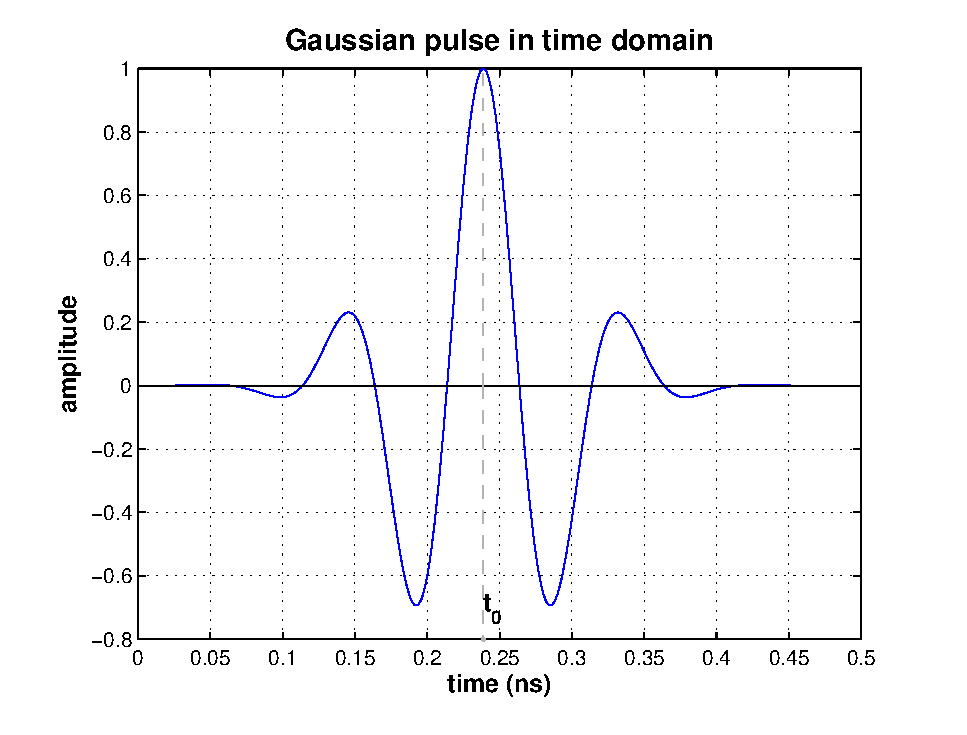
\includegraphics[width=0.48\textwidth]{svg/GaussPulseTime.eps}} 
	      \subfloat[In frequency domain]{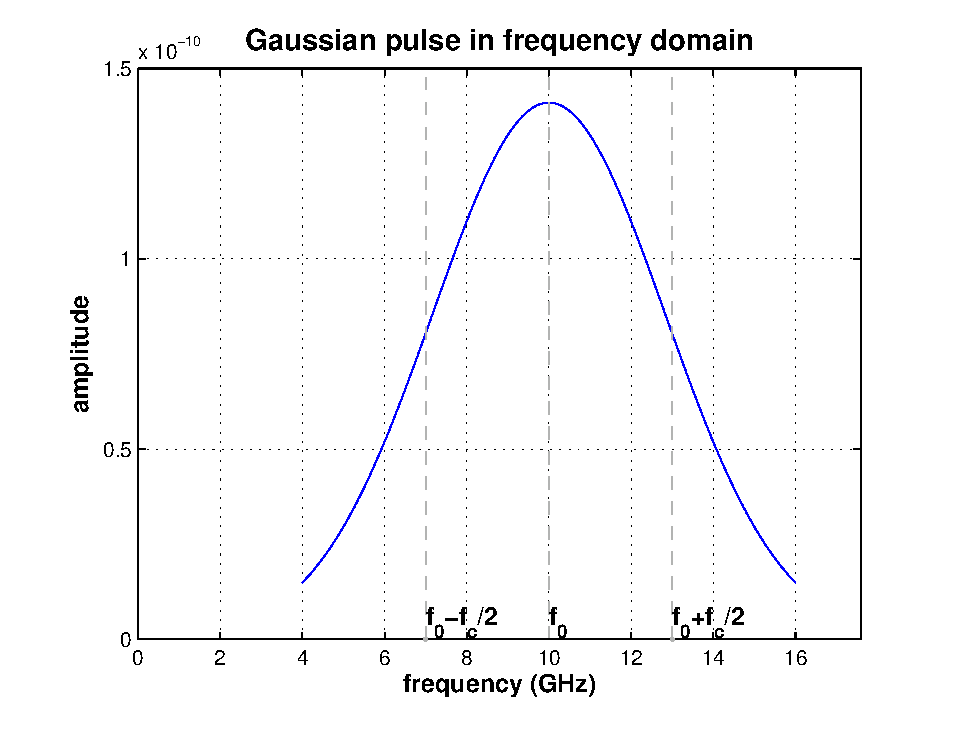
\includegraphics[width=0.48\textwidth]{svg/GaussPulseFreq.eps}}\\
	      \subfloat[In dB]{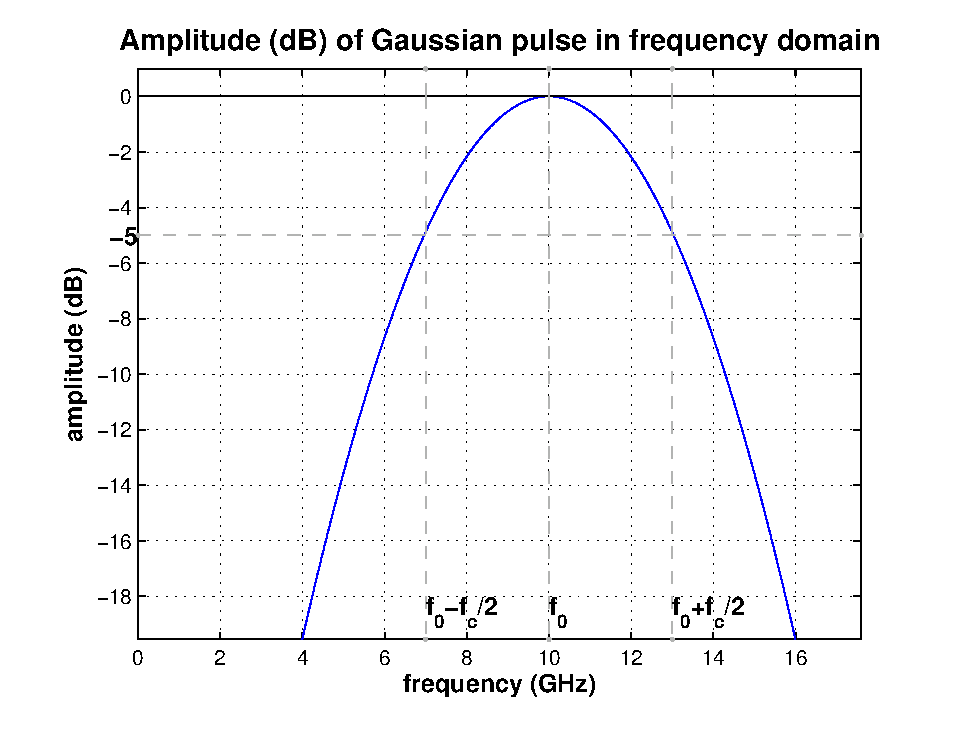
\includegraphics[width=0.48\textwidth]{svg/GaussPulseFreqdB.eps}} 
	      \caption[Gaussian pulse signal]{An instance of Gaussian pulse signal with $f_0=10GHz \quad f_c=6GHz$}
	      \label{fig:GaussInpulseTheory}
    \end{figure}
According to the expression \ref{equ:GussianSignal_freq}, a Gaussian signal can be defined with function \hyperref[func:SetGaussExcite]{\texttt{SetGaussExcite(FDTD,f0,fc)}}.

%%%%%%%%%%%%%%%%%%%%%%% FUNCTION  SetGaussExcite %%%%%%%%%%%%%%%%
\textcolor{blue}{\begin{large}\textbf{SetGaussExcite}	\end{large}}\phantomsection \label{func:SetGaussExcite}\\
	  Set a Gaussian function as the signal of the excitation.

\textcolor{blue}{\begin{large}Syntax:\end{large}}
 \begin{lstlisting}
FDTD = SetGaussExcite(FDTD,f0,fc)
 \end{lstlisting}

\textcolor{blue}{\begin{large}Definition:\end{large}}\\
      This function update the structure \hyperref[para:FDTD]{\texttt{FDTD}} with the expression \ref{equ:GussianSignal_freq}. 

\textcolor{blue}{\begin{large}Description:\end{large}}\\
%%%%%%%%%%%%%%%%%%%%%%%%%%%% FDTD
	\hyperref[para:FDTD]{\texttt{FDTD}} 
	    \begin{myindentpar}
		A structure in MATLAB. See \hyperref[para:FDTD]{\texttt{FDTD}}.
	    \end{myindentpar}
%%%%%%%%%%%%%%%%%%%%%%%%%%%% f0
	\texttt{f0}  \phantomsection \label{para:f0} %\hyperref[para:f0]{\texttt{f0}} 
	    \begin{myindentpar}
		\hyperref[para:f0]{\texttt{f0}}  is the frequency of the modulating co-sinusoidal signal. It's also the central frequency of the Gaussian signal. At this frequency the signal has the highest amplitude or energy. 
	    \end{myindentpar}
%%%%%%%%%%%%%%%%%%%%%%%%%%%% fc
	\texttt{fc}  \phantomsection \label{para:fc} %\hyperref[para:fc]{\texttt{fc}} 
	    \begin{myindentpar}
		\hyperref[para:fc]{\texttt{fc}} determines the variance of the signal. It is a central bandwidth. In the band [\hyperref[para:f0]{\texttt{f0}}-\hyperref[para:fc]{\texttt{fc}}/2 \quad \hyperref[para:f0]{\texttt{f0}}+\hyperref[para:fc]{\texttt{fc}}/2] the signal is greater then about -5dB. See figure \ref{fig:GaussInpulseTheory}. And the maximal frequency to be simulated is \hyperref[para:f0]{\texttt{f0}}+\hyperref[para:fc]{\texttt{fc}}.The greater \hyperref[para:fc]{\texttt{fc}} is, the flater is the signal in frequency domain, but cliffier and shorter in time domain.
	    \end{myindentpar}
\warning{Too small \hyperref[para:fc]{\texttt{fc}} will lead to a time-consuming simulation. Too great \hyperref[para:fc]{\texttt{fc}} will lead to a signal in a very short time relative to a time step. Both cases should be advoided.}

%%%%%%%%%%%%%%%%%%%%% Examples.	  
	\textcolor{blue}{\begin{large}Examples:\end{large}}\\
\begin{itemize}
\item An Gaussian pulse with a central frequency \hyperref[para:f0]{\texttt{f0}}=0.5GHz, and a -5dB bandwidth of \hyperref[para:fc]{\texttt{fc}}=0.5GHz. 
\begin{lstlisting}
% Initiation of FDTD 
FDTD = InitFDTD(5000,1e-5,'OverSampling',10);
% Update FDTD with a  Gaussian pulse excitation. 
% f0=0.5GHz, fc=0.5GHz
FDTD = SetGaussExcite(FDTD,0.5e9,0.5e9);
% The field  FDTD.Excitation.ATTRIBUTE  has been assigned.
\end{lstlisting}
Under this setting, a Gaussian pulse has been set up. And the signal reduces to -5dB at 0.25GHz and 0.75GHz. The maximal frequency in simulation is 1GHz.
\end{itemize}

%%%%%%%%%%%%%%%%%%%%%%%%%%%%%%%%%%%% subsection Sinousoidal signal %%%%%%%%%%%%%%%%%%%%%%%%%%%%%%%%%%%%%%%%%%%%%%%%%%%%%%%%%%%%%%%%%%%%%
    \subsection{Sinousoidal signal}\label{subsec:Sinousoidal signal}
\textcolor{blue}{\begin{large}\textbf{SetSinusExcite}	\end{large}}\phantomsection \label{func:SetSinusExcite}\\
	  Set a sinusoidal function as the signal of the excitation.

\textcolor{blue}{\begin{large}Syntax:\end{large}}
 \begin{lstlisting}
FDTD = SetSinusExcite(FDTD,f0)
 \end{lstlisting}

\textcolor{blue}{\begin{large}Definition:\end{large}}\\
      The signal in time domain has an form as following function\\
\begin{equation}\label{equ:SinusoidalSignal_time}
 f(t)=\sin{(2\pi f_0t)}, \text{ for } t>0
\end{equation}

\textcolor{blue}{\begin{large}Description:\end{large}}\\
%%%%%%%%%%%%%%%%%%%%%%%%%%%% FDTD
	\hyperref[para:FDTD]{\texttt{FDTD}} 
	    \begin{myindentpar}
		A structure in MATLAB interface. See \hyperref[para:FDTD]{\texttt{FDTD}}.
	    \end{myindentpar}
%%%%%%%%%%%%%%%%%%%%%%%%%%%% f0
	\texttt{f0}  \phantomsection \label{para:sin_f0} %\hyperref[para:sin_f0]{\texttt{f0}} 
	    \begin{myindentpar}
		\hyperref[para:sin_f0]{\texttt{f0}}  is the unique frequency of the homonic signal. 
	    \end{myindentpar}

%%%%%%%%%%%%%%%%%%%%% Examples.	  
	\textcolor{blue}{\begin{large}Examples:\end{large}}\\
\begin{itemize}
\item A sinousoidal signal with a  frequency \hyperref[para:sin_f0]{\texttt{f0}}=0.5GHz. 
\begin{lstlisting}
% Initiation of FDTD 
FDTD = InitFDTD(5000,1e-5,'OverSampling',10);
% Assignment for f0
f0=0.5e9;
% Update FDTD with a sinousoidal excitation. 
FDTD = SetSinusExcite(FDTD,f0);
% The field  FDTD.Excitation.ATTRIBUTE
% has been assigned.
\end{lstlisting}
A sinousoidal excitation with frequency 0.5GHz has been set up in OpenEMS. 
\end{itemize}

%%%%%%%%%%%%%%%%%%%%%%%%%%%%%%%%%%%% subsection excitation signals %%%%%%%%%%%%%%%%%%%%%%%%%%%%%%%%%%%%%%%%%%%%%%%%%%%%%%%%%%%%%%%%%%%%%
    \subsection{Other excitation signals}\label{subsec:Other excitation signals}
OpenEMS provides various kinds of excitation signals. Besides the Gaussian pulse and sinusoidal signal, it has also other forms of excitation, such as dirac function, step function and even custom function. Here is the introduction of how to set up an excitation with any custom function by using \hyperref[func:SetCustomExcite]{\texttt{SetCustomExcite}}.

\textcolor{blue}{\begin{large}\textbf{SetCustomExcite}	\end{large}}\phantomsection \label{func:SetCustomExcite}\\
	  Set a custom function as the signal of the excitation.

\textcolor{blue}{\begin{large}Syntax:\end{large}}
 \begin{lstlisting}
FDTD = SetCustomExcite(FDTD,f0,funcStr)
 \end{lstlisting}

\textcolor{blue}{\begin{large}Definition:\end{large}}\\
      The signal in time domain is a function like the given string \texttt{funcStr}.

\textcolor{blue}{\begin{large}Description:\end{large}}\\
%%%%%%%%%%%%%%%%%%%%%%%%%%%% FDTD
	\hyperref[para:FDTD]{\texttt{FDTD}} 
	    \begin{myindentpar}
		A structure in MATLAB. See \hyperref[para:FDTD]{\texttt{FDTD}}.
	    \end{myindentpar}
%%%%%%%%%%%%%%%%%%%%%%%%%%%% f0
	\texttt{f0}  \phantomsection \label{para:custom_f0} %\hyperref[para:f0]{\texttt{f0}} 
	    \begin{myindentpar}
		\hyperref[para:f0]{\texttt{f0}}  is the nyquist rate. 
	    \end{myindentpar}
%%%%%%%%%%%%%%%%%%%%%%%%%%%% funcStr
	\texttt{funcStr}  \phantomsection \label{para:custom_funcStr} %\hyperref[para:custom_funcStr]{\texttt{funcStr}} 
	    \begin{myindentpar}
		\hyperref[para:custom_funcStr]{\texttt{funcStr}}   is a string of an expression in MATLAB. This expression is of \texttt{t}, the time. It denotes how is the function of excitation.  And two constants can be used directly in the expression, \texttt{e} for Euler's number and \texttt{pi} for $\pi$. Futher more any strings of defined valuables can be used in \hyperref[para:custom_funcStr]{\texttt{funcStr}}.
	    \end{myindentpar}

%%%%%%%%%%%%%%%%%%%%% Examples.	  
	    \textcolor{blue}{\begin{large}Examples:\end{large}}\\
    \begin{itemize}
	\item A ramped sinus excite 
	\begin{lstlisting}
% Initiation of FDTD 
FDTD = InitFDTD(5000,1e-5,'OverSampling',10);
% The nyquist rate f0=1GHz
f0=1e9;
% Time step is of the nyquist rate f0
T = 1/f0;
% Update FDTD with a given string 
% of an excitation expression of t. 
FDTD = SetCustomExcite(FDTD,f0, ...
       [ '(1-exp(-1*(t/' num2str(T) ...
        ')^2) ) * sin(2*pi*'  ...
        num2str(f0) '*t)' ]);
% The field  FDTD.Excitation.ATTRIBUTE 
% has  been assigned.
	\end{lstlisting}
    \end{itemize}
 

%%%%%%%%%%%%%%%%%%%%%%%%%%%%%section Boundary Conditions%%%%%%%%%%%%%%%%%%%%%%%%%%%%%%%%%%%%%%%%%%%%%%%%%%%%%%%%%%%%
%%%%%%%%%%%%%%%%%%%%%%%%%%%%%%%%%%%%%%%%%%%%%%%%%%%%%%%%%%%%%%%%%%%%%%%%%%%%%%%%%%%%%%%%%%%%%%%%%%%%%%%%%%%%%%%%%%
%%%%%%%%%%%%%%%%%%%%%%%%%%%%%section Boundary Conditions%%%%%%%%%%%%%%%%%%%%%%%%%%%%%%%%%%%%%%%%%%%%%%%%%%%%%%%%%%%%
%%%%%%%%%%%%%%%%%%%%%%%%%%%%%%%%%%%%%%%%%%%%%%%%%%%%%%%%%%%%%%%%%%%%%%%%%%%%%%%%%%%%%%%%%%%%%%%%%%%%%%%%%%%%%%%%%%
\section{Boundary Conditions}\label{sec:BC}
%%%%%%%%%%%%%%%%%%%%%%%%%%%%%%%%%%%% subsection General introduction to boundary conditions %%%%%%%%%%%%%%%%%%%%%%%%%%%%%%%%%%%%%%%%%%%%%%%%%%%%%%%%%%%%%%%%%%%%%
    \subsection{General introduction to boundary conditions}\label{subsec:General introduction to BC}
    \subsubsection{Equations of boundary conditions}\label{subsubsec:Equations of BC}
	  Boundary conditions (BC) are necessary for solving the  Maxwell's equations by FDTD. They can limit the computation in a finite space but attaining the same solution just as in a infinite one.  \\
	  The following equations are the general boundary conditions at an arbitrary interface of two medium. And there can be  charges (denoted as charge density $\rho_s$) or  currents (denoted as surface electric current density $\vec{\mathbf{J}}_s$ and  surface magnetic current density $\vec{\mathbf{M}}_s$) at the interface:
	  %%%%% BC EQ
	      \begin{eqnarray}
		  \hat{n}\cdot(\vec{\mathbf{D}}_2-\vec{\mathbf{D}}_1) &=&\rho_s  \\
		  \hat{n}\cdot(\vec{\mathbf{B}}_2-\vec{\mathbf{B}}_1) &=&0  \\
		  \hat{n}\times(\vec{\mathbf{E}}_2-\vec{\mathbf{E}}_1) &=&-\vec{\mathbf{M}}_s \\
		  \hat{n}\times(\vec{\mathbf{H}}_2-\vec{\mathbf{H}}_1) &=&\vec{\mathbf{J}}_s
		  \label{eq:General boundary conditions}
	      \end{eqnarray}
      %     %%%%% BC Diagrams
      %     Figure  \ref{fig:General BC diagrams} shows the above relations.
      %     \begin{figure}[ht]
      %       \centering
      % 	  %\subfloat[CAPTION]{BILDERCODE}\qquad
      % 	  \subfloat[$\vec{\mathbf{D}}$]{\includegraphics[width=0.4\textwidth]{svg/BC_general_Dn.eps}}\qquad
      % 	  \subfloat[$\vec{\mathbf{B}}$]{\includegraphics[width=0.4\textwidth]{svg/BC_general_Bn.eps}}\qquad 
      % 	  \subfloat[$\vec{\mathbf{E}}$]{\includegraphics[width=0.4\textwidth]{svg/BC_general_Et.eps}}\qquad
      % 	  \subfloat[$\vec{\mathbf{H}}$]{\includegraphics[width=0.4\textwidth]{svg/BC_general_Ht.eps}}\qquad 
      % 	    \caption[General BC diagrams]{General boundary condition on an interface between 2 media for $\vec{\mathbf{D}}$, $\vec{\mathbf{B}}$, $\vec{\mathbf{E}}$ and $\vec{\mathbf{H}}$. n denotes normal components. t denotes tangential components. s denotes surface.}
      % 	    \label{fig:General BC diagrams}
      %     \end{figure}
    \subsubsection{Four particularly useful types of boundary conditions in OpenEMS}\label{subsubsec:Four particularly usefull BC}
	Under some special given conditions or assumptions, the boundary conditions(\ref{eq:General boundary conditions}) have  respective forms and they are convenient for the most simulations. These BC are called as perfect electric conductor (\textbf{PEC}), perfect magnetic conductor (\textbf{PMC}), \textbf{MUR} absorbing boundary condition and perfectly matched layer (\textbf{PML}) absorbing boundary condition. More details of these four types of BC are  given in the following subsections (\ref{subsec:PEC}, \ref{subsec:PMC}, \ref{subsec:MUR} and  \ref{subsec:PML}). And the types of these BC are represented as a field of the structure  \hyperref[para:FDTD]{\texttt{FDTD}} in MATLAB. And it's named as \texttt{BoundaryCond}. \phantomsection \label{para:BoundaryCond}
    \subsubsection{Setting boundary conditions in OpenEMS with function SetBoundaryCond}\label{subsubsec:Setting boundary conditions in OpenEMS with function SetBoundaryCond}
	\textcolor{blue}{\begin{large}\textbf{SetBoundaryCond}	\end{large}}\\
	  Setting boundary conditions for simulation. Assigning the field \hyperref[para:BoundaryCond]{\texttt{BoundaryCond}} of structure \hyperref[para:FDTD]{\texttt{FDTD}}  in MATLAB.

        \textcolor{blue}{\begin{large}Syntax:\end{large}}
 \begin{lstlisting}
FDTD = SetBoundaryCond(FDTD, BC)
%or with advanced arguments
FDTD = SetBoundaryCond(FDTD, BC, varargin)
 \end{lstlisting}

	\textcolor{blue}{\begin{large}Description:\end{large}}\\
	\hyperref[para:FDTD]{\texttt{FDTD}}
  \begin{myindentpar}\hyperref[para:FDTD]{\texttt{FDTD}}  is a structure in Matlab. It contains 3 fields:
       \begin{myindentpar}\texttt{ATTRIBUTE} \\
	      \texttt{Excitation} \\
	      \texttt{BoundaryCond}
      \end{myindentpar}
  \end{myindentpar}
%%%%%%%%%%%%%%%%%%%%%%%%%%%% BC
	\texttt{BC}  
\begin{myindentpar}\texttt{BC} provides the types of the boundary conditions to the 6 boundaries of the 3D simulating space.  
          \texttt{BC} is defined either as a \textbf{vector} or as a \textbf{cell} with 6  elements. \vspace{2mm}\\
          If  T\_xmin,T\_xmax,T\_ymin,T\_ymax,T\_zmin and T\_zmax are  arguments which denote for the types of the conditions at the respective boundaries, then \texttt{BC} can be defined as a vector or a cell as following.\vspace{2mm}\\
       %%%%%%%%%%%% vector BC
          \texttt{BC} is defined as a \textbf{vector}
	\begin{myindentpar}
% 	  \lstset{caption={\texttt{BC} in the form of a vector},label=BCinvector}
	  \begin{lstlisting}[caption={\texttt{BC} in the form of a vector},label=BCinvector]
 BC=[T_xmin T_xmax T_ymin T_ymax T_zmin T_zmax]; 
	  \end{lstlisting}
          And   each  element(T\_?min or T\_?max)  must be set as one of the following numbers 
	    \begin{myindentpar}
	      \textcolor{green}{\texttt{0}}   \qquad  (represents for PEC)\\
	      \textcolor{green}{\texttt{1}}   \qquad  (represents for PMC)\\
	      \textcolor{green}{\texttt{2}}   \qquad  (represents for MUR)\\
	      \textcolor{green}{\texttt{3}}   \qquad  (represents for PML with 8 layers).
	    \end{myindentpar}	
      \end{myindentpar}  
          %%%%%%%%%%%% Cell BC      		                                                                     
          Or \texttt{BC} is defined as a \textbf{cell} 
	  \begin{myindentpar}
% 	   \lstset{caption={\texttt{BC} in the form of a cell},label=BCincell}
	  \begin{lstlisting}[caption={\texttt{BC} in the form of a cell},label=BCincell]
 BC={T_xmin T_xmax T_ymin T_ymax T_zmin T_zmax};
	  \end{lstlisting}
	  of which   each  element(T\_?min or T\_?max)  must be set as one of the following strings 
	  \begin{myindentpar}
	     \textcolor{green}{\texttt{'PEC'}} \qquad   (represents for PEC)\\
	     \textcolor{green}{\texttt{'PMC'}} \qquad   (represents for PMC)\\
	     \textcolor{green}{\texttt{'MUR'}}  \qquad  (represents for MUR)\\
	     \textcolor{green}{\texttt{'PML\_x'}} \qquad   (represents for PML. \texttt{x} is  the PML size. It should be replaced with an integer in an interval from 4 to 50).
	  \end{myindentpar}	
	\end{myindentpar}	
	  So the element \texttt{BC}($i$) or \texttt{BC}\{$i$\} represents for the type of the  condition at the respective boundary as showed in the following table
	  \begin{table}[htb]\centering
	  \begin{tabular}{l|l}
	  \texttt{BC($i$)} or \texttt{BC\{$i$\}} & Respective position of the boundary\\ \hline
		 \texttt{BC(1)} or  \texttt{BC\{1\}} & where x or $\rho$ is minimum\\
		 \texttt{BC(2)} or  \texttt{BC\{2\}}& where x or $\rho$ is maximum\\
		 \texttt{BC(3)} or  \texttt{BC\{3\}}& where y or $\varphi$ is minimum\\
		 \texttt{BC(4)} or  \texttt{BC\{4\}}& where y or $\varphi$is maximum\\
		 \texttt{BC(5)} or  \texttt{BC\{5\}}& where z is minimum\\
		 \texttt{BC(6)} or  \texttt{BC\{6\}}& where z is maximum
	  \end{tabular}\caption{The elements represent for the types of conditions at the boundaries.}
	  \end{table}
	  \label{Elements of BC and the rescpective boundaries}.
         \end{myindentpar}
            %%%%%%%%%%%%%%%% Info 
	\info{In a cylindrical system,  the elements of \texttt{BC} represent for the types of boundary conditions respective at $\rho$, $\varphi$, z instead of x, y, z(see listing \ref{ListingCylinBC}). If there are no  BC at $\rho\_min=0$ or at $\varphi$,  then the elements of  \texttt{BC} for respective boundaries conditions   can be set as \texttt{0} or \texttt{'PEC'} just in a virtual form for computation(see listing \ref{listing:SettingofBC in a cylin.}). For these cases, the respective elements have nothing to do with the boundaries conditions indeed. } \\
% 	  \lstset{caption={\texttt{BC} in a cylindrical coordinate},label={ListingCylinBC}}
         \begin{lstlisting}[caption={\texttt{BC} in a cylindrical coordinate},label={ListingCylinBC}]
% as a vector
  BC=[T_rhomin T_rhomax T_phimin T_phimax T_zmin T_zmax];
% as a cell
  BC={T_rhomin T_rhomax T_phimin T_phimax T_zmin T_zmax}
	  \end{lstlisting}%%question: phi_min and phi_max don't form a closed circle,then???
%%%%%%%%%%%%%%%%%%%%%% varargin
	      Advanced arguments \texttt{Varargin}:
      \begin{myindentpar} \texttt{Varargin}  are  arguments of advanced settings. They can be either neglected or replaced with the following alternative arguments  
		\begin{myindentpar}
		  \textcolor{green}{\texttt{'MUR\_PhaseVelocity'}}\\
		  \textcolor{green}{\texttt{'PML\_Grading'}}\\
		  \textcolor{green}{\texttt{'gradFunction'}}.
		\end{myindentpar}
      and respective values following them.\vspace{2mm}\\
			%%%%%%%%%%%%%% MUR
		\texttt{'MUR\_PhaseVelocity'} 
		  \begin{myindentpar}
		      It defines a phase-velocity to be used by the MUR-abc
		      useful e.g. for dispersive waveguides
		  \end{myindentpar}
	    \vspace{2mm} 
			%%%%%%%%%%%%%%% PML
	      \texttt{'PML\_Grading'} or \texttt{'gradFunction'} 
		\begin{myindentpar}
		They define the PML grading function.\vspace{2mm}
			    Predefined variables in this grading function are:
			      \begin{myindentpar}
				D  = depth in the pml in meter\\
				dl = mesh delta inside the pml in meter\\
				W  = width (length) of the pml in meter\\
				N  = number of cells for the pml\\
				Z  = wave impedance at the current depth and position
			    \end{myindentpar}
		\end{myindentpar}
      \end{myindentpar}

%%%%%%%%%%%%%%%%%%%%% Examples.	  
	\textcolor{blue}{\begin{large}Examples:\end{large}}\\
\begin{itemize}
%%%%%%%1st step
 \item    Setting boundary conditions in a Cartesian coordinate system.\\
       1st step: \texttt{BC} assignment
    \begin{myindentpar}
	  \begin{lstlisting}[caption={BC assignment as fig \ref{fig:Ex. 1st of SetBoundaryCond} },label={listing:1st SettingofBC}]
	  %using numbers 
	  BC=[ 1     1     0     0     2     3     ] 
	  %or using equivalent strings
	  BC={'PMC' 'PMC' 'PEC' 'PEC' 'MUR' 'PML_8'} 
		      \end{lstlisting}
	  Both above vector and cell set  the x-boundaries(perpendicular to x axis) as PMC, and the y-boundaries(perpendicular to y axis) as PEC, the zmin-boundary(perpendicular to z axis and z is minimum) as MUR but the zmax-boundary(perpendicular to z axis and z is maximum) as PML with 8 layers. These boundary condition are showed in fig \ref{fig:Ex. 1st of SetBoundaryCond}.
	      \begin{figure}[ht]
		      \centering
		    \subfloat[BC at x and y]{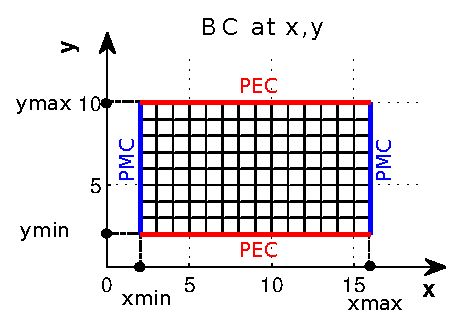
\includegraphics[width=0.4\textwidth]{svg/BCXY1.eps}}\qquad
		    \subfloat[BC at x and z]{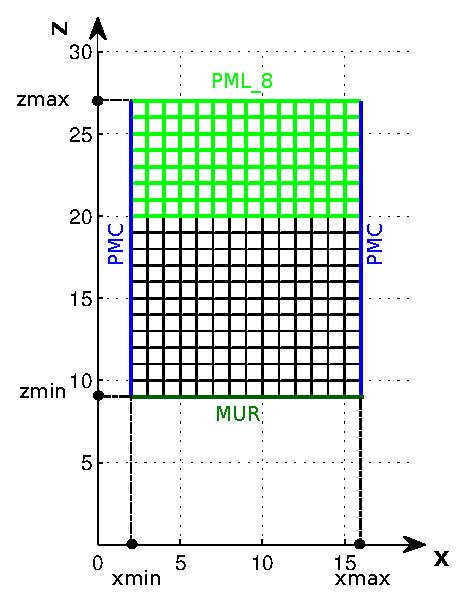
\includegraphics[width=0.4\textwidth]{svg/BCXZ1.eps}}\qquad 
%\includegraphics[width=0.9\textwidth]{svg/BCXY.eps}
		      \caption[1st example for the setting of boundary conditions]{\texttt{BC=[1 1  0 0  2 3]} ,see listing \ref{listing:1st SettingofBC}}
		      \label{fig:Ex. 1st of SetBoundaryCond}
		\end{figure}
    \end{myindentpar}
%%%%%%%2nd step
      2nd step: Updating the \hyperref[para:FDTD]{\texttt{FDTD}} structure with BC or other andvanced arguments.
      \begin{myindentpar}	    
		    \begin{lstlisting}
  % without advanced arguments
  FDTD=SetBoundaryCond(FDTD,BC); 
		    \end{lstlisting}
		      or
		    \begin{lstlisting}
  % with advanced argument for MUR
  FDTD=SetBoundaryCond(FDTD,BC,...
       'MUR_PhaseVelocity',300000000);
			\end{lstlisting}
		    \begin{lstlisting}
  % with advanced argument for PML
  FDTD=SetBoundaryCond(FDTD,BC,...
       'PML_Grading','-log(1e-6)*log(2.5)/...
       (2*dl*pow(2.5,W/dl)-1)*pow(2.5, D/dl)/Z');
		    \end{lstlisting}	 
    \end{myindentpar}	
%%%%%%%%%% cylindrical sys
 \item Setting boundary conditions in a cylindrical coordinate system.\\
If there are no boundaries at  $\rho_{min}=0$ and at any $\varphi$, then please set the elements as \texttt{0} or \texttt{'PEC'} as the following example.
    \begin{lstlisting}[caption={BC assignment in a cylindrical coordinate system as fig \ref{fig:Ex. SetBoundaryCond in cylin.}},label={listing:SettingofBC in a cylin.}]
	% no boundaries at rhomin=0 , phi_min and phi_max
	BC=[0 1 0 0 3 3];
	%or using equivalent strings
	%BC={'PEC' 'PMC' 'PEC' 'PEC' 'PML_8' 'PML_8'} 
	FDTD=SetBoundaryCond(FDTD,BC); 
			\end{lstlisting} 
    \begin{figure}[ht]
			  \centering
			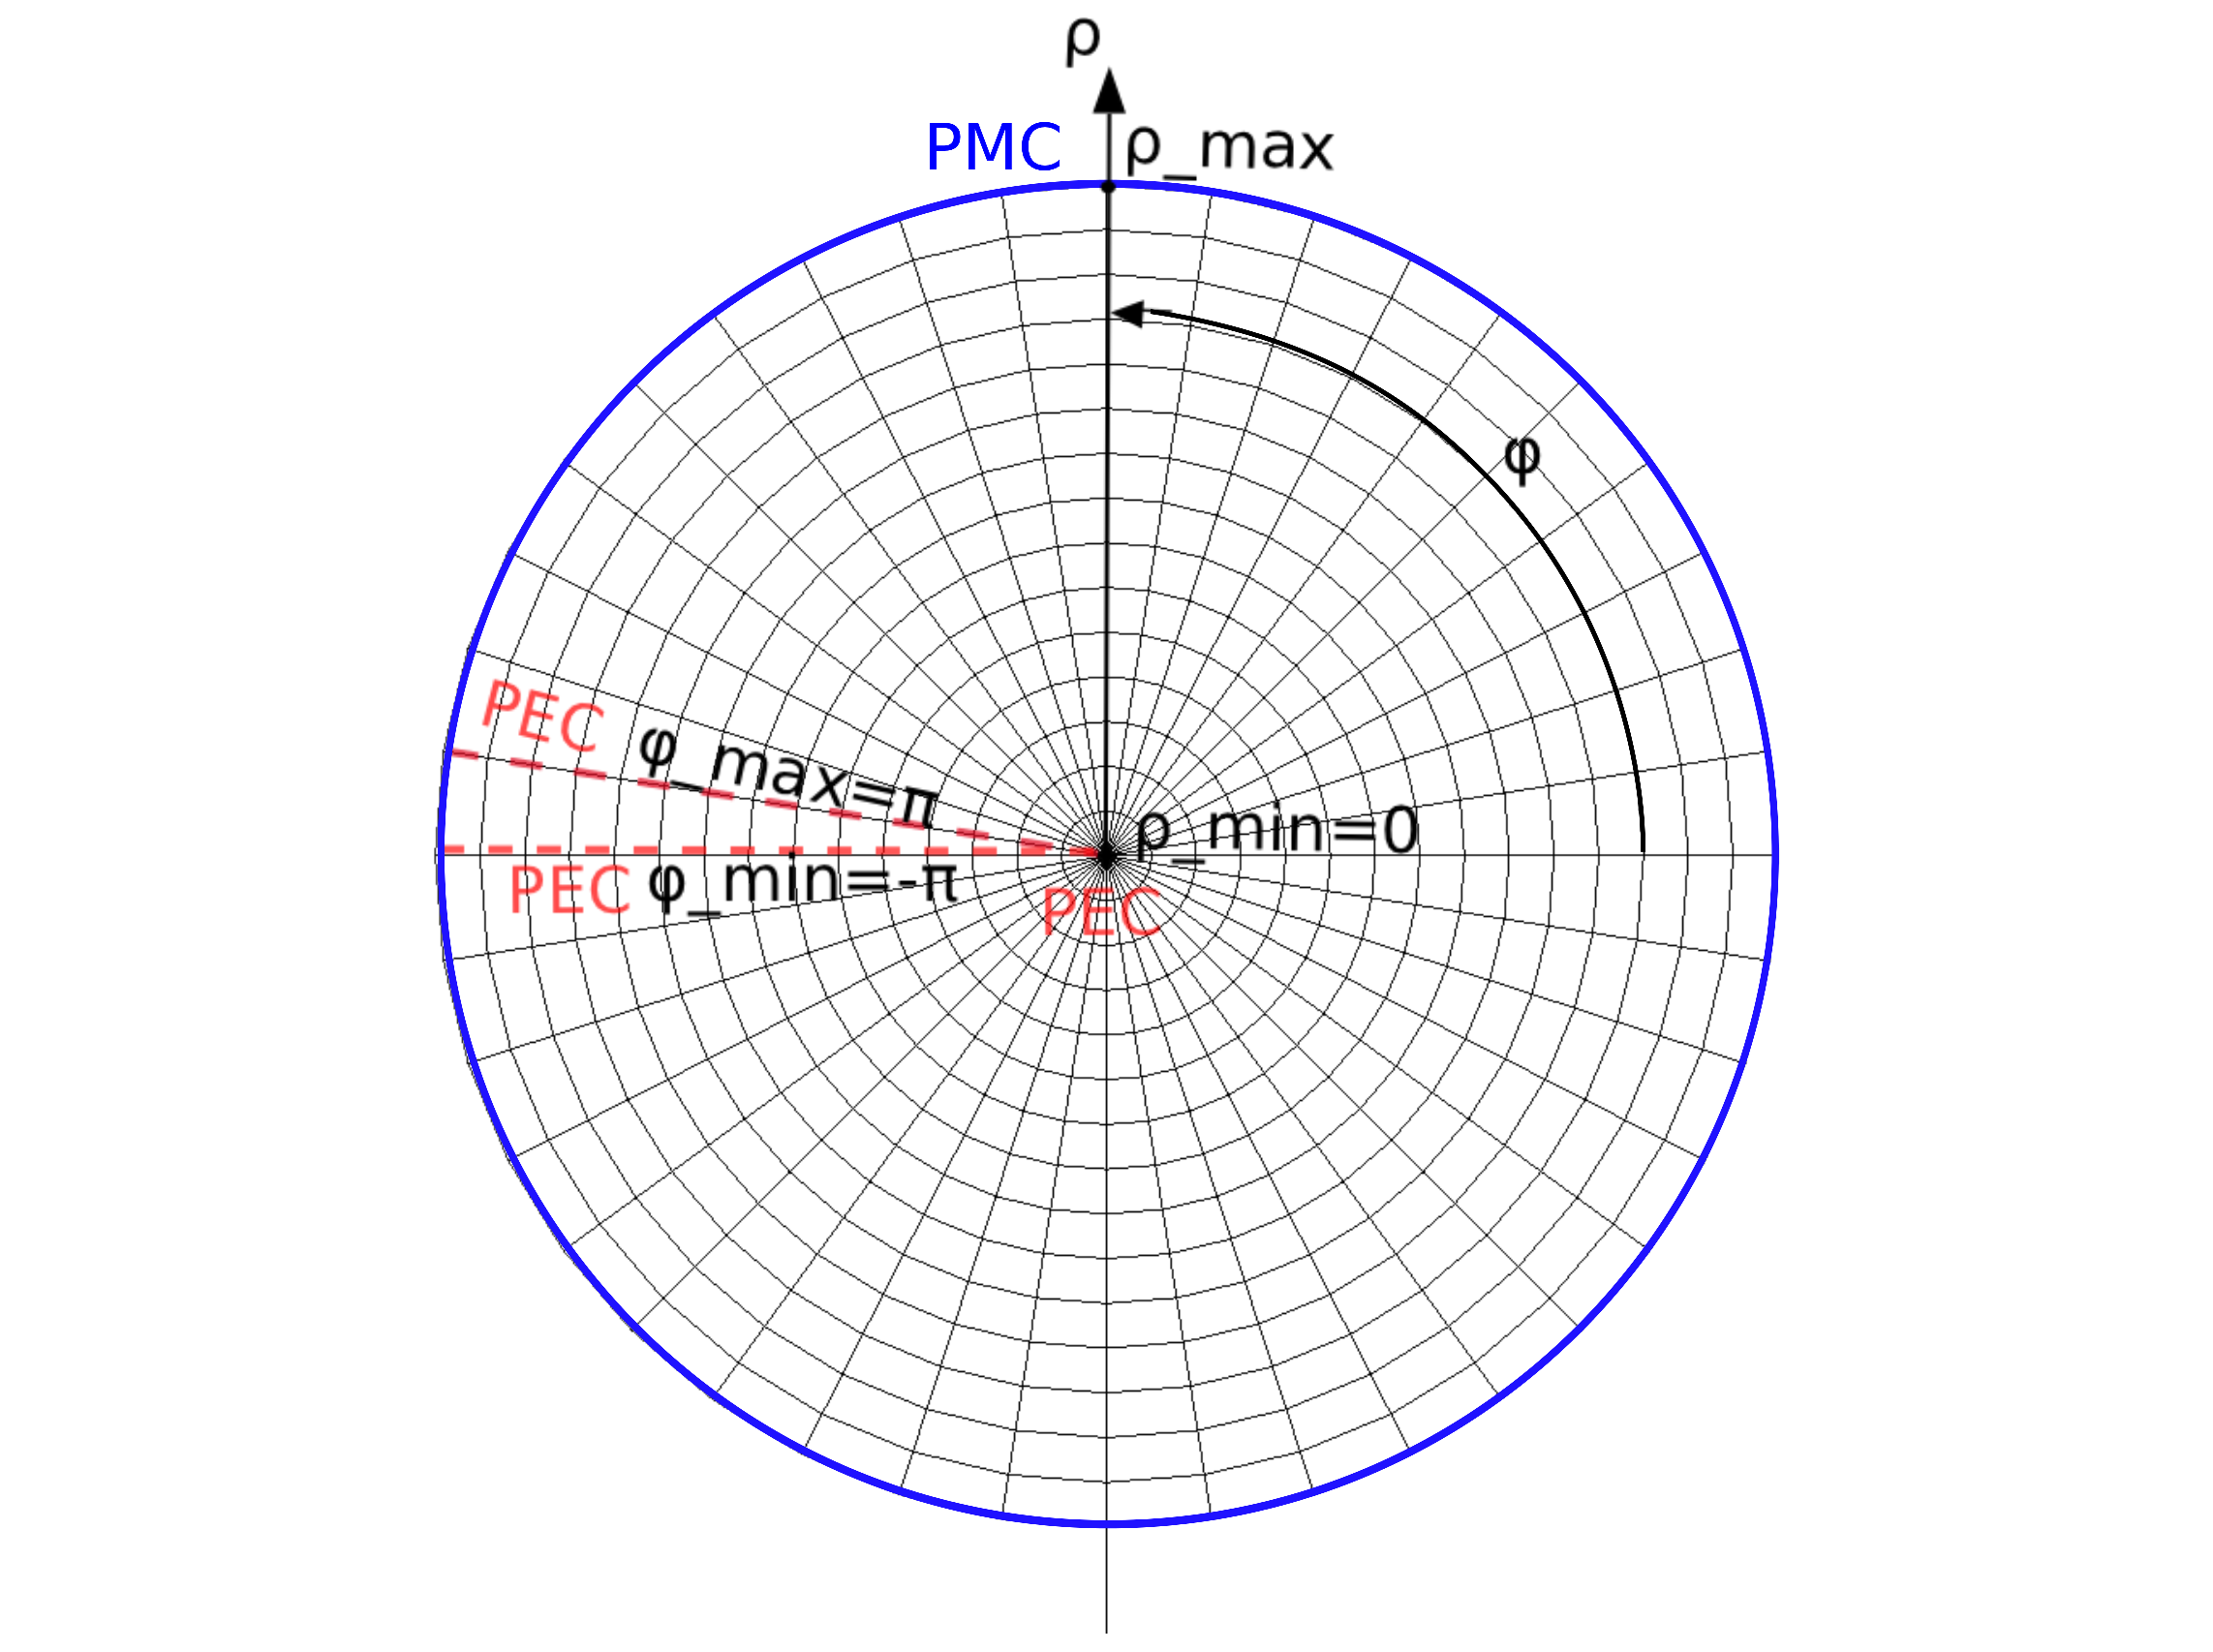
\includegraphics[width=0.6\textwidth]{svg/CylinBCXY.eps}\qquad
			  \caption[ Setting virtual boundary conditions in a cylindrical coordinate system]{Virtual boundary conditions in a cylindrical coordinate system. See listing \ref{listing:SettingofBC in a cylin.}}
			  \label{fig:Ex. SetBoundaryCond in cylin.}
		    \end{figure}
%%%%%%%%%%%%% half cylindrical
If there are boundaries at $\rho_{min}\neq0$ and $\varphi$, then please set the elements as respective number or string.
\begin{lstlisting}[caption={BC assignment in a cylindrical coordinate system as fig \ref{fig:Ex. SetBoundaryCond in cylin. Half}},label={listing:SettingofBC in a cylin. Half}]
	% no boundaries at rhomin=0 , phi_min and phi_max
	BC=[0 1 0 1 0 3];
	%or using equivalent strings
	%BC={'PEC' 'PMC' 'PEC' 'PMC' 'PEC' 'PML_8'} 
	FDTD=SetBoundaryCond(FDTD,BC); 
			\end{lstlisting} 
    \begin{figure}[H]
			  \centering
 \subfloat[Boundaries conditions at $z$  ]{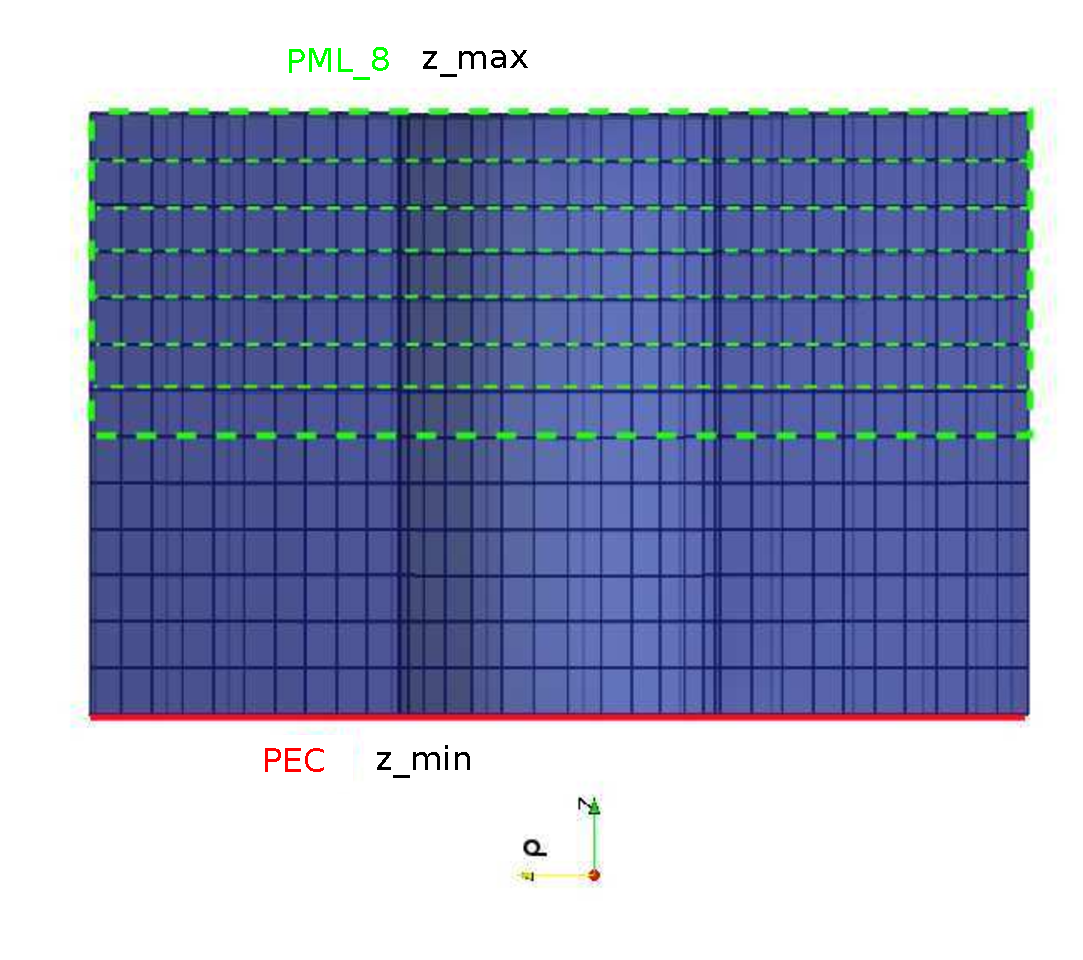
\includegraphics[width=0.6\textwidth]{svg/CylinBCXZ2.eps}}\qquad
 \subfloat[ Boundaries conditions at $\rho$ and $\varphi$ ]{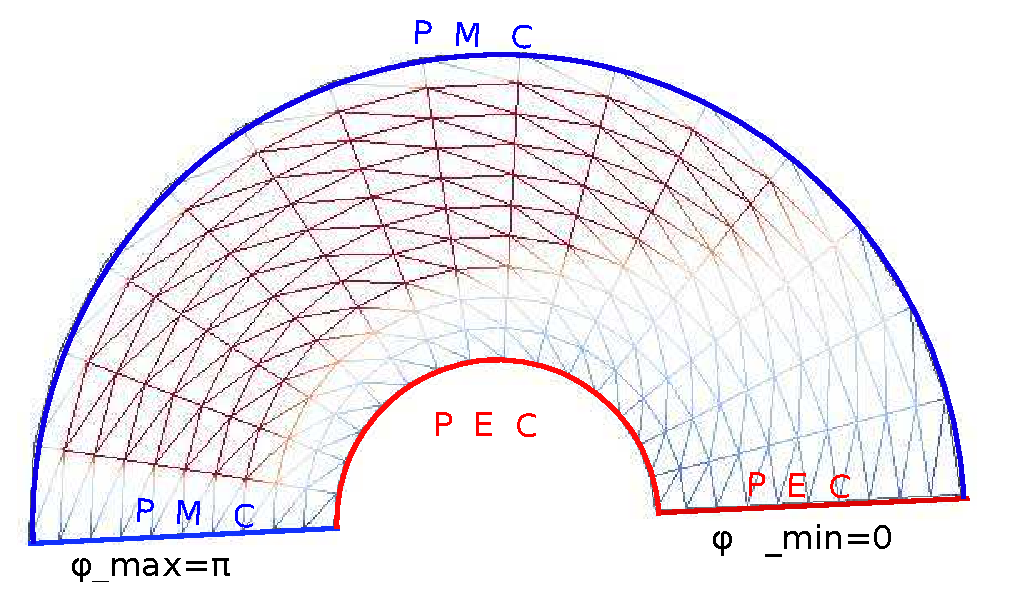
\includegraphics[width=0.55\textwidth]{svg/CylinBCXY2.eps}}\qquad 
			  \caption[ Setting  boundary conditions in a cylindrical coordinate system]{An example of boundary conditions in a cylindrical coordinate system. See listing \ref{listing:SettingofBC in a cylin. Half}}
			  \label{fig:Ex. SetBoundaryCond in cylin. Half}
		    \end{figure}
\end{itemize}
%%%%%%%%%%%%%%%%%%%%%%%%%%%%%%%%%%%% subsection Perfect electric conductor (PEC) %%%%%%%%%%%%%%%%%%%%%%%%%%%%%%%%%%%%%%%%%%%%%%%%%%%%%%%%%%%%%%%%%%%%%
    \subsection{Perfect electric conductor (PEC)}\label{subsec:PEC}
    \subsubsection{Definition of PEC}
    If one media beside the boundary is theoretically lossless(conductivity $\sigma\rightarrow\infty$, or so called \textbf{perfect conductor}), then the BC can be expressed as
	%%%%% PEC BC EQ
	    \begin{eqnarray}
		\hat{n}\cdot\vec{\mathbf{D}}_1 &=&-\rho_s  \\
		\hat{n}\cdot\vec{\mathbf{B}}_1 &=&0  \\
		\hat{n}\times\vec{\mathbf{E}}_1 &=&0\\
		\hat{n}\times\vec{\mathbf{H}}_1 &=&-\vec{\mathbf{J}}_s .
		\label{eq:PEC boundary conditions}
	    \end{eqnarray}
    \subsubsection{The condition for application of PEC}
    In practice, this BC can be applied where the media  is \textbf{good conductor(e.g., metal)}, because the good conductor can often be seen as nearly lossless(perfect). So condition for using PEC can be summarized as either
    \begin{itemize}
    \item one media is good conductor(e.g., metal) \\
    or
    \item $\sigma\rightarrow\infty$.
    \end{itemize}
    \subsubsection{The Setting of PEC in OpenEMS}

    %     %%%%% PEC BC Diagrams
    %     Figure  \ref{fig:PEC BC diagrams} shows the above relations.
    %     \begin{figure}[ht]
    %             \centering
    % 	    \includegraphics[width=0.4\textwidth]{svg/PEC_BC_general_Dn.eps}
    % 	    \caption[PEC BC diagrams]{PEC boundary condition  for $\vec{\mathbf{D}}$, $\vec{\mathbf{B}}$, $\vec{\mathbf{E}}$ and $\vec{\mathbf{H}}$. n denotes normal components. t denotes tangential components. s denotes surface.}
    % 	    \label{fig:PEC BC diagrams}
    %     \end{figure}
\warning{The first or last layer of nodes of E field in the boundary can not be updated, because there are no enough nodes of H field around them for calculation. So the field there should be neglected.}

%%%%%%%%%%%%%%%%%%%%%%%%%%%%%%%%%%%%%%%%%%%%%%%%% subsection Perfect magnetic conductor (PMC) %%%%%%%%%%%%%%%%%%%%%%%%%%%%%
\subsection{Perfect magnetic conductor (PMC)}\label{subsec:PMC}
H perpendicular to BC

%%%%%%%%%%%%%%%%%%%%%%%%%%%%%%%%%%%%%%%%%%%%%%%%% subsection MUR absorbing boundary condition %%%%%%%%%%%%%%%%%%%%%%%%%%%%%
\subsection{MUR absorbing boundary condition}\label{subsec:MUR}

%%%%%%%%%%%%%%%%%%%%%%%%%%%%%%%%%%%%%%%%%%%%%%%%% subsection Perfectly matched layer (PML) absorbing boundary condition %%%%%%%%%%%%%%%%%%%%
\subsection{Perfectly matched layer (PML) absorbing boundary condition}\label{subsec:PML}
matched--impedance ,no reflection , for infinite  material, an virtual BC for computation
\warning{Since the field is absorbed in the boundary artificially, please pay attention to any setting in these region. For example, don't place any excitation in it. And please set enough layers of meshes, such that the boundary works correctly.}

